%Summer Paper version2 summerv2.tex
\documentclass[12pt]{article}
\usepackage{amssymb,latexsym}
\usepackage[round,sort]{natbib}
\usepackage{multirow,array}
\usepackage{fancyhdr}
\usepackage{lastpage}
\usepackage{graphicx}
\usepackage[bottom]{footmisc}
\graphicspath{ {summerv2-images/} }
\usepackage[T1]{fontenc}
\usepackage{mathptmx}
\usepackage{tabu}
\usepackage{textcomp}
\usepackage{stata}
\usepackage{listings}
\usepackage{hyperref}
\hypersetup{
    colorlinks=true,
    linkcolor=blue,
    filecolor=magenta,      
    urlcolor=cyan,
}
\newenvironment{hypothesis}{
  	\itshape
  	\leftskip=\parindent \rightskip=\parindent
  	\noindent\ignorespaces}

\pagestyle{fancy}
\fancyhf{}
\lhead{Investigating the pattern of knowledge flows across regions}
\rfoot{Page \thepage  \ of \pageref{LastPage}}
\rhead{Iyenggar}

\begin{document}
\title{Investigating the pattern of knowledge flows across regions:\\  Evidence from US patent data}
\author{Ashwin Iyenggar  (1521001) \\ ashwin.iyenggar15@iimb.ernet.in} 


\maketitle
\thispagestyle{empty}

\begin{abstract}
I document the steps followed in transforming the raw patents data from patentsview.org to suit our analysis of knowledge flow patterns across geographic regions. In doing so, I also highlight assumptions and potentially debatable decisions on data selection and culling. The investigation clearly differentiates the two MSAs of San Francisco-Oakland-Hayward, CA and San Jose-Sunnyvale-Santa Clara, CA as demonstrating much higher levels of knowledge spillovers after normalization. Additionally, the locations from emerging countries in our sample, Bangalore, Beijing and Israel exhibit very low levels of local knowledge spillovers.
\end{abstract}

\section{Introduction}\label{S:Introduction}
Our objective in this project is to investigate the patterns of knowledge flow as evidenced by patent citations across geographic regions around the world. The motivation for doing so comes from the fact that a lot of theory about knowledge spillovers have their empirical basis from data from certain technological clusters in the United States. We wish to test the theory over a wider setting and potentially contribute to the extant theory by better understanding the heterogeneity that characterizes different regions. 

\section{Objectives}
We have set ourselves the objective of evaluating the nature of knowledge flows across geographic regions by initially looking at six major regions of the world: San Francisco and greater Bay Area of California, Austin, Texas, the greater Boston area, Tel Aviv, Beijing and Bangalore. The sampling has been made keeping in mind both established and upcoming technological locations. In order to proceed with empirical work, it is necessary to determine a certain line of investigation. For the current iteration of this project, those decisions are as follows.  First, Analysis will be focussed on a region of interest, and flows will be measured over time. Second, flows will be mapped on the two dimensions of region (geography) and beneficiary. Along each axis we are interested in local and internal flows as against global and external flows of knowledge. Finally, in order that the various regions may be compared on these axes, the flows of knowledge within each quadrant will be normalized to a percent value of the total flows for that region that year.

\section{Definition of Geographic Regions}
I discuss here how I go about defining the geographic regions of interest to this investigation.  For locations in the United States, it is standard to use Metropolitan Statistical Areas (MSA) for analyses related to economic geography. The approach is less standard for non-US locations, and this problem is particularly exacerbated by the absence of a similar measure as the MSA. Urban areas are a reasonable substitute for  economic centers, and we therefore determine to use one such definition. Specifically, for MSA of US locations, I obtain data from \href{http://www.census.gov/geo/maps-data/data/cbf/cbf_msa.html}{the US census} and for urban areas for world wide locations, I obtain data from \href{http://www.naturalearthdata.com/downloads/10m-cultural-vectors/}{Natural Earth Data}.
 
This automatically raises conflicting definitions for locations in the United States. So that the MSA definitions take precedence, I eliminated all data pertaining to US locations from the Natural Earth urban centers data and integrated this with the MSA information. With this I  generated a single database of location information for economic centers around the world. The appendix provides visual map-based snapshots of our regions of interest. The regions colored yellow are the ones in focus, while those in purple are neighboring regions outside the region of interest. 

\begin{table}
\begin{centering}
\begin{tabular}{|c|c|}
\hline
\textbf{Category}&\textbf{Number of citations}\\\hline
cited by applicant&16,527,942\\\hline
cited by examiner&17,174,252\\\hline
cited by other&25,444,463\\\hline
cited by third party&325\\\hline
&21,581,784\\\hline
\end{tabular}
\caption {Categories of patent citations}
\label{table:uspatentcitation}
\end{centering}
\end{table} 

We note from the MSA data that the Bay Area of California is actually split between the two MSA regions of San Francisco-Oakland-Hayward, CA and San Jose-Sunnyvale-Santa Clara, CA. I therefore decide to treat the two as two regions for the current analysis. It is possible that we may need analyze the data again clubbing the two in the future. Bangalore is seen as including Hosur, the Boston-Cambridge-Newton MSA includes parts of New Hampshire and Beijing seems to extend a bit to the south.  These seem to be reasonable definitions for the respective economic geographies. 

\section{Mapping geographical co-ordinates to regions}
The file named \verb|location.tsv| from patentsview.org contains the latitude and longitude information for all locations referenced in the patentsview.org database. The \verb|location.tsv| associates a \verb|location_id| to each latitude-longitude combination. I use the merged MSA and urban centers information and the geographical information in \verb|location.tsv| to obtain a mapping from each \verb|location_id| used in the patentsview database to the economic geography that it corresponds to. The patentsview.org database defines 128,911 unique location\_ids, and our data is able to map 53,424 of those locations to an economic geography region. The rest are assumed to be those locations that fall outside any major urban center in the world from which patents from been filed or been assigned.

\section{Selecting applicant cited patent citations}
The \verb|uspatentcitation.tsv| file from patentsview.org maps every patent-patent level citation that has been made since 1976. This file has 80,728,766 observations. Table ~\ref{table:uspatentcitation} provides a break up based on category. The US patent office has been systematically categorizing citations by category since after the year 2000. This explains the many empty citation category entries. 


In order that we are consistent with our initial objective of measuring only applicant cited patents as flows of knowledge, we restrict ourselves to those patents categorized as 'cited by applicant'. This decision has the additional effect of limiting our period of analysis to citing patents applied for after the year 2000. 
\begin{table}
\begin{centering}
\begin{tabular}{|c|c|}
\hline
\textbf{Region}&\textbf{Number of citations}\\\hline
Boston-Cambridge-Newton, MA-NH&4,602,355\\\hline
San Jose-Sunnyvale-Santa Clara, CA&8,431,536\\\hline
Bangalore&183,685\\\hline
Beijing&131,752\\\hline
Tel Aviv-Yafo&872,578\\\hline
San Francisco-Oakland-Hayward, CA&9,258,684\\\hline
Austin-Round Rock, TX&259,503\\\hline
\end{tabular}
\caption {Number of citation entries by region of interest (till 2012)}
\label{table:selected-citations}
\end{centering}
\end{table}
\section{Expanding the US patent citation}
I use the \verb|application.tsv| file to determine the year of application of the citing patent and then use this to add a year field to the uspatentcitation entry. After selecting only those citation entries where the year of application of the citing patent is 2012 or earlier, we are left with 11,822,154 citation entries. In order to determine internal firm flows or external firm flows of knowledge, I use the assignee\_id on each patent to identify similarity or dissimilarity of assignees. There are 5,300,888 unique assignee entries. While a vast majority of patents are assigned to a single assignee, there are a few that are assigned to more than one assignee. In attaching assignee\_id to each citing and cited patent on a citation, I create separate entries for each unique assignee on each patent. With this we end up with 12,256,759 citation entries of which 2,869,978 entries have an empty assignee\_id for either the citing patent or the cited patent. A future revision could potentially work to reduce the loss due to empty assignee\_id. The 12,256,759 citation entries with year and assignee\_ids for both citing and cited patents are then expanded to include every inventor on each citing patent and each cited patent. This process is performed using a Python script as the joinby process was turning out to be extremely time consuming on \stata (I had runs of over 40 hours without \stata finishing). At the end of this process, I had 105,369,401 citing-patent-assignee-location to cited-patent-assignee-location citation entries. This formed the master dataset for the further analysis.

\section{Analysis of flows}\label{S:Analysis}
Table ~\ref{table:selected-citations} captures the number of citing patent-inventor-assignee to cited patent-inventor-assignee flows that form the dataset on which further investigation is conducted. 


\begin{figure}[h]
\begin{centering}
  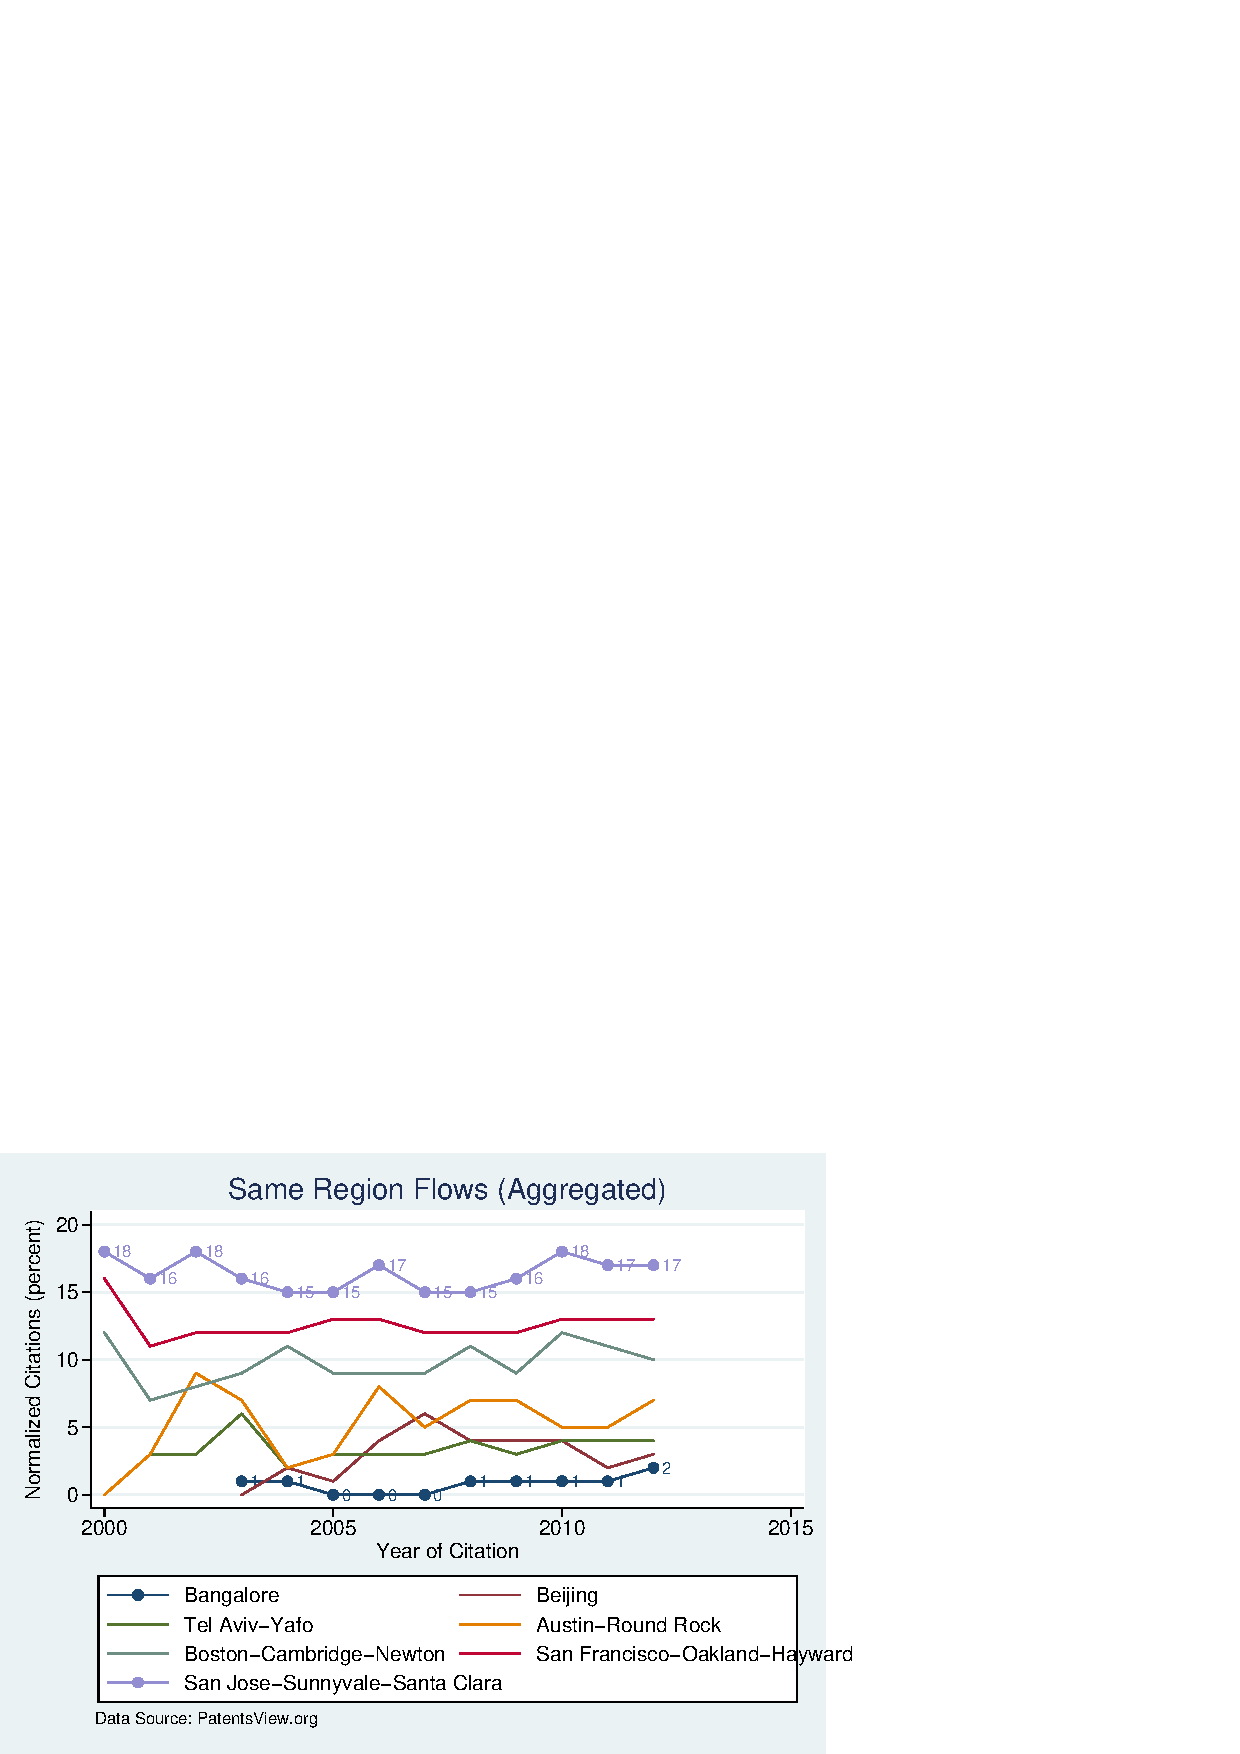
\includegraphics[width=\textwidth]{SameRegionFlows}
  \caption{Local Knowledge Flows by Region}
  \label{fig:SameRegionFlows}
\end{centering}
\end{figure}

\begin{figure}[h]
\begin{centering}
  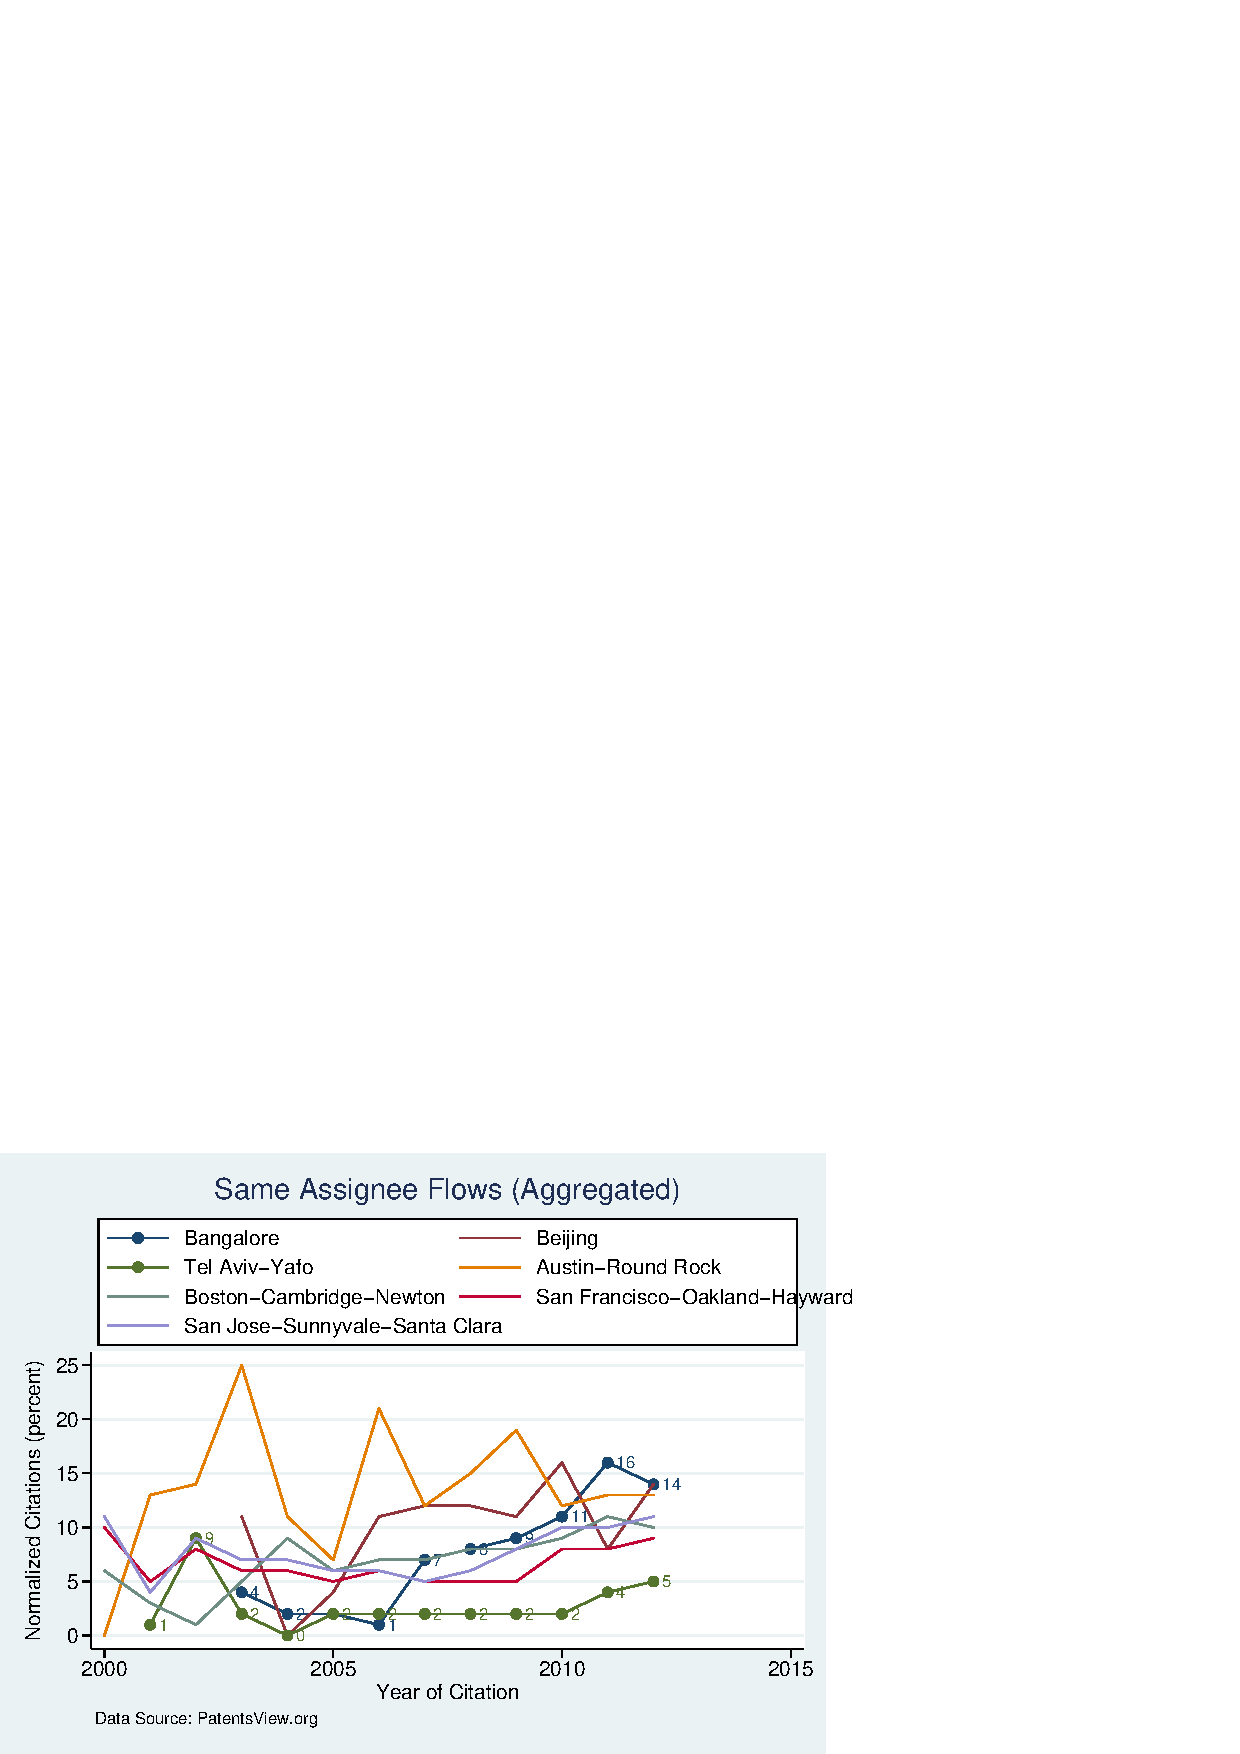
\includegraphics[width=\textwidth]{SameAssigneeFlows}
  \caption{Internal Knowledge Flows by Region}
  \label{fig:SameAssigneeFlows}
\end{centering}
\end{figure}

Starting with 23,825,110 entries, we drop duplicate citations between the same patents and the same regions. This leaves us with 5,820,864 entries. In determining if the citing patent assignee and the cited patent assignee match, we drop all those entries where assignee information is unavailable for either side. That leaves us with  5,058,782 entries. We similarly drop those entries where either location region is unknown. We do so because it would seem incorrect to conclude that two locations differ when one location is undefined. After this step, we have 4,661,422 entries in our data set where conclusions can be clearly made about whether the assignees match and if the locations match between citing patent inventors and cited patent inventors. With this dataset, we calculate the normalized scores in our 2x2, and two aggregate measures - the first for same location flows across assignees, and the second for same assignee flows across locations. All six scores are expressed in percentages rounded to the nearest integer. The results are plotted in linear scale and are evident in the following graphs.



\begin{figure}[h]
\begin{centering}
  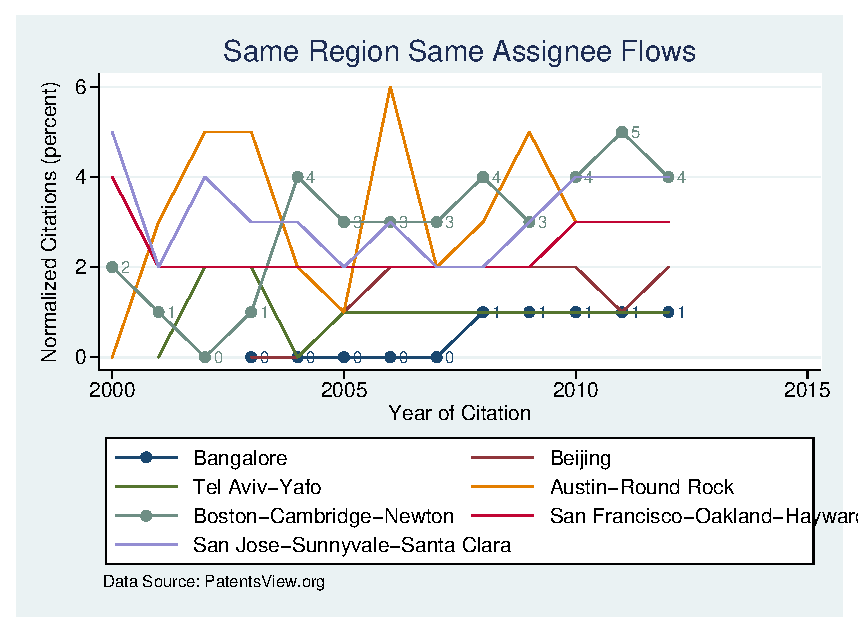
\includegraphics[width=\textwidth]{SameRegionSameAssigneeFlows}
  \caption{Local and Internal Flows by Region}
  \label{fig:SameRegionSameAssigneeFlows}
\end{centering}
\end{figure}

\begin{figure}[h]
\begin{centering}
  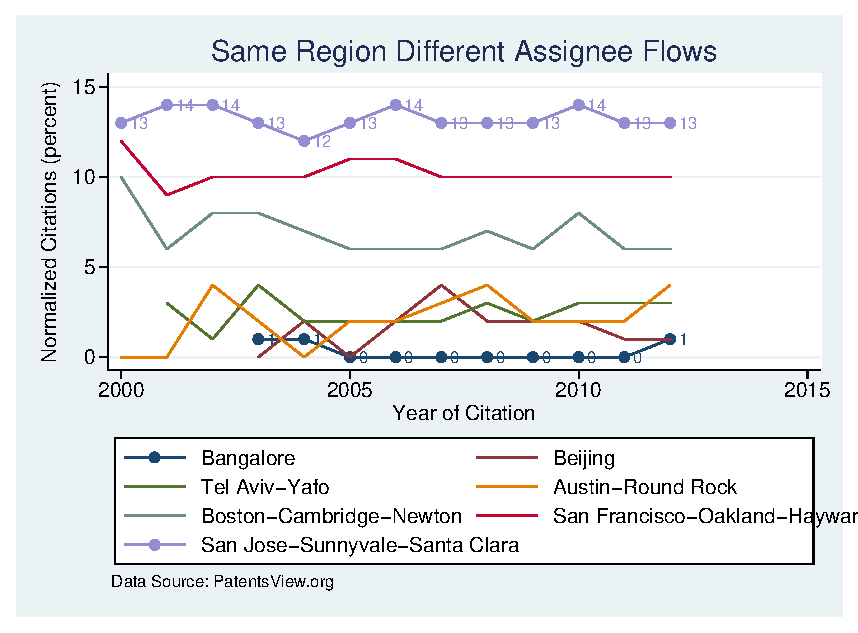
\includegraphics[width=\textwidth]{SameRegionDiffAssigneeFlows}
  \caption{Local and External Flows by Region}
  \label{fig:SameRegionDiffAssigneeFlows}
\end{centering}
\end{figure}

\section{Preliminary results}
Figure ~\ref{fig:SameRegionFlows} clearly indicates that the phenomenon of knowledge spillovers is strongly evident in the two California locations in our sample, and to a smaller extent in the extended Boston region. But clearly, the localization of knowledge spillovers is not observed in the three emerging country locations of Bangalore, Tel Aviv and Beijing. Figure {fig:SameRegionDiffAssigneeFlows} reiterates the gulf between the two California locations and the rest. On the other hand from Figure ~\ref{fig:SameAssigneeFlows}, we note that the Bangalore region has seen an increasing share of flows to non-local but internal flows. This maybe proof of an increasing amount of research being done in Bangalore by global multinationals for their corporate headquarters. It is also interesting to note that while Beijing and Bangalore are at a similar level (14 percent) in 2012 on this count, Bangalore has seen a steady increase while Beijing has somewhat stalled since 2005.

Additionally Figure ~\ref{fig:DiffRegionDiffAssigneeFlows} demonstrate the stark difference between Tel Aviv-Yafo and San Jose-Sunnyvale-Santa Clara, CA on the extent of non-local external flows. Tel Aviv-Yafo seems to be strongly integrated into the external knowledge network but not at all locally. Figure ~\ref{fig:DiffRegionSameAssigneeFlows} reiterates the Bangalore position as the outsourcing destination for global R\&D, and also Tel Aviv insignificant impact in this dimension.


\begin{figure}[h]
\begin{centering}
  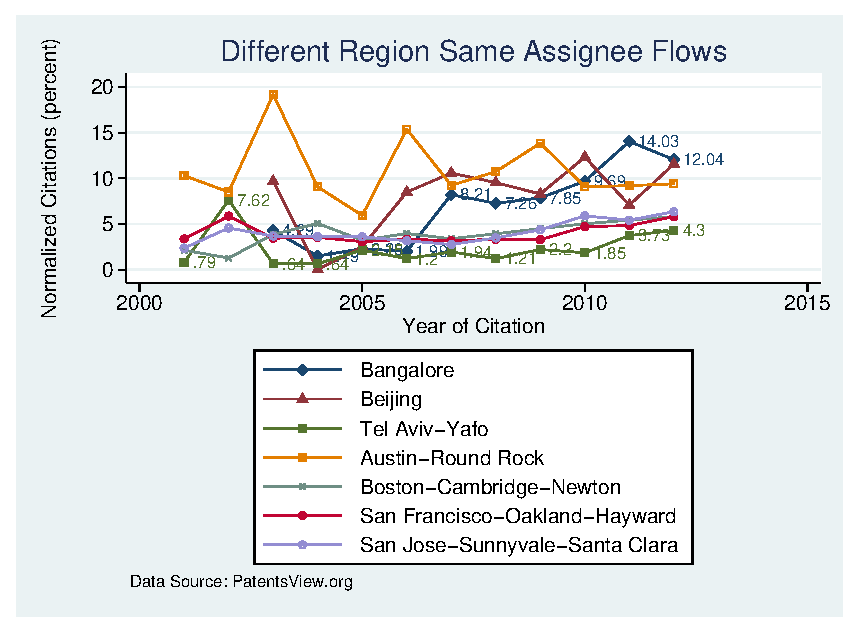
\includegraphics[width=\textwidth]{DiffRegionSameAssigneeFlows}
  \caption{Non-local and Internal Flows by Region}
  \label{fig:DiffRegionSameAssigneeFlows}
\end{centering}
\end{figure}

\begin{figure}[h]
\begin{centering}
  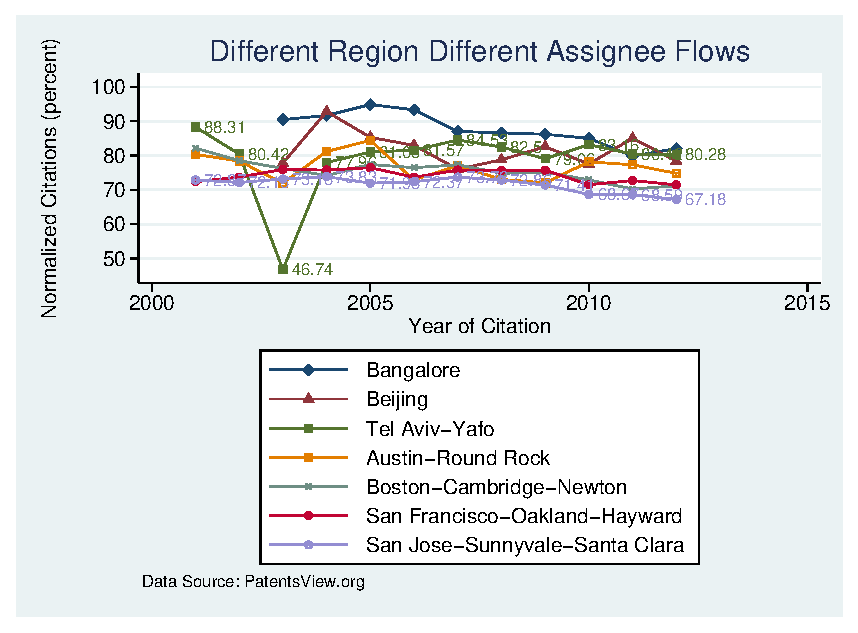
\includegraphics[width=\textwidth]{DiffRegionDiffAssigneeFlows}
  \caption{Non-local and External Flows by Region}
  \label{fig:DiffRegionDiffAssigneeFlows}
\end{centering}
\end{figure}

\newpage
\appendix

\section{Spatial Data}

\begin{figure}[h]
\begin{centering}
  \includegraphics[width=\textwidth]{Austin}
  \caption{Geographic Definition of Austin-Round Rock, TX}
   \label{fig:Austin}
\end{centering}
\end{figure}

\begin{figure}[h]
\begin{centering}
  \includegraphics[width=\textwidth]{Bangalore}
  \caption{Geographic Definition of Bangalore}
   \label{fig:Bangalore}
\end{centering}
\end{figure}

\begin{figure}[h]
\begin{centering}
  \includegraphics[width=\textwidth]{Beijing}
  \caption{Geographic Definition of Beijing}
   \label{fig:Beijing}
\end{centering}
\end{figure}

\begin{figure}[h]
\begin{centering}
  \includegraphics[width=\textwidth]{Boston}
  \caption{Geographic Definition of Boston-Cambridge-Newton, MA-NH}
   \label{fig:Boston}
\end{centering}
\end{figure}

\begin{figure}[h]
\begin{centering}
  \includegraphics[width=\textwidth]{SanFrancisco}
  \caption{Geographic Definition of San Francisco-Oakland-Hayward, CA}
   \label{fig:SanFrancisco}
\end{centering}
\end{figure}

\begin{figure}[h]
\begin{centering}
  \includegraphics[width=\textwidth]{SanJose}
  \caption{Geographic Definition of San Jose-Sunnyvale-Santa Clara, CA}
   \label{fig:SanJose}
\end{centering}
\end{figure}

\begin{figure}[h]
\begin{centering}
  \includegraphics[width=\textwidth]{TelAviv}
  \caption{Geographic Definition of Tel Aviv-Yafo}
   \label{fig:TelAviv}
\end{centering}
\end{figure}

\end{document}
